\documentclass[a4paper,12pt]{ctexbook}
\usepackage[margin=2cm]{geometry}
\usepackage{graphicx}
\usepackage{subfigure}
\usepackage{float}
\usepackage[colorlinks,linkcolor=black]{hyperref}%colorlinks启用链接颜色,linkcolor指定对应的颜色
\usepackage{listings}
%\usepackage[cache=false]{minted}  % 代码高亮X
\usepackage{fontspec}
\usepackage{tikz,xcolor,mwe}


\definecolor{cvgreen}{HTML}{92D14F}
\definecolor{cvgray}{HTML}{D8E4BE}
\definecolor{cvtext}{HTML}{92909B}
\usetikzlibrary{shadows}

\pagestyle{empty}
\CTEXsetup[format={\Large\bfseries}]{section}%可以让section的标题左对齐。
%\CTEXsetup[format+={\flushleft}]{section}%让section的标题居左
%\renewcommand{\thesection}{\chinese{section}}%将“1.1”改为汉字“一”,但是subsection就会变成  六.1 ,比较难看,还是不用比较好。

\begin{document}
\begin{tikzpicture}[remember picture,overlay] 
\fill[cvgreen] (current page.north west) rectangle ([xshift=6cm]current page.south west);% green bar
\fill[cvgray] ([yshift=-11cm]current page.north west) rectangle ([yshift=-17cm]current page.north east); % gray bar

\node[cvtext,right] at ([xshift=3.5cm,yshift=-13cm]current page.north west) {\Huge Study \LaTeX};
\node[cvtext,above left] at ([xshift=-1cm,yshift=-16.5cm]current page.north east) {\Large\bfseries \today};
% cover photo
\node[inner sep=0pt,below right] (image) at ([xshift=17cm,yshift=-1cm]current page.north west) {
\includegraphics[width=3cm]{hainulogo.png}};
% name and address
\node[fill=white,align=center,text width=6.4cm,inner sep=0.8cm,below] (name) at (image.south) {};
\node[text width=15cm,inner sep=0.3cm,below right] at (name.south west){\Large Author:Flynn\\E-Mail:zofon@qq.com};
% attachments
\node[white,text width=5cm,inner sep=0.6cm,above right] at ([yshift=1cm]current page.south west)
{\large\obeylines\textbf{This is for \\The Hi-Net Group}};  
\end{tikzpicture}

\tableofcontents

\begin{flushleft}

\chapter{学习准备}
\section{\LaTeX 介绍~\cite{1994Latex}}
latex是一个排版软件,和Microsoft Office Word 等所见即所得的办公软件不同,用\LaTeX 排版文档,
首先要用文本编辑器编辑好tex 文档,然后通过各种程序编译,得到pdf 文档用于打印或者阅读。一般我们经常用pdflatex
或者xelatex 程序直接从tex文件生成pdf文件。如果是中文tex文档,优先使用xelatex程序编译。如图~\ref{LaTex的基本的排版流程}:
\begin{figure}[H]
\centering
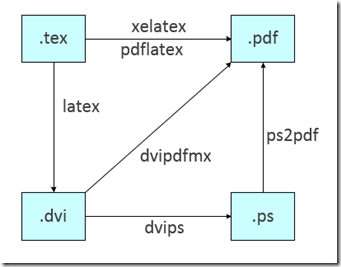
\includegraphics[width=6cm]{Figures/latex_build.png}
\label{LaTex的基本的排版流程}
\caption{LaTex的基本的排版流程}	
\end{figure}
在\hyperref{http://www.latexstudio.net/}{category}{LaTex开源小屋}{LaTex开源小屋}中有很多相关的资源。


\section{关于编辑器和编译平台}
在windows环境下,ctex是最好的选择,然后使用WinEdt作为编辑器最好。

在linux环境下,编辑器一般是TexStudio(推荐使用)或者vim。要安装tex相关的软件。命令如下:
\begin{verbatim}
sudo apt-get install texlive-full
\end{verbatim}


\chapter{开始编写文档}
我将这一节的内容放在基础语法的前面,目的是让大家快速的上手,先写出文档,如果遇到不会的内容,就接着往下看。
\section{确定文档的类型}
文档的类型由\verb|\documentclass[a4paper,12pt]{ctexbook}|决定,可以看到,
本文档的类型为ctexbook,也就是书籍的类型,一般的教程之类的文档可以使用这样的文档类型。下面列举几个可用的文档类型:
\begin{itemize}
	\item \verb|\documentclass[a4paper,12pt]{book}|,书籍类型,只能识别英文,中文会乱码。
	\item \verb|\documentclass[a4paper,12pt]{ctexbook}|,可以编译中文的文档。
	\item \verb|\documentclass[a4paper,12pt]{article}|,文章类型的文档,同理,不能识别中文。
	\item \verb|\documentclass[a4paper,12pt]{ctexart}|,文章类型,可以识别中文。
\end{itemize}

\section{设置页边距的大小}
在本文中,页面距离设置为2cm,设置如下:\verb|\usepackage[margin=2cm]{geometry}|

\section{文章的内容}
这部分就是文章的正文,如果正文中需要插入图片,请参考~\ref{picture_position}\\
如果文章中想添加一些抄录的内容,可以参考~\ref{verbatim}\\
文章中需要用到数学公式的时候,请参考~\ref{define_function}和~\ref{superscript}

\section{添加文献的引用}
文献的引用有几种方法,在windows下的时候和linux不一样:
\subsection{使用Bitex方法}
首先编写bib文件,这个文件编写之后在用之前是要编译一下的。

命令如下:\verb|bibtex FengZhou-MPTCP|

然后在文档的下方加入如下命令:
\begin{verbatim}
\bibliographystyle{IEEEtran.bst}%表示指定文献引用的格式
\bibliography{ReferenzarchivWithoutURLs,OtherReferences}%对应的引用文件。
\end{verbatim}

\subsection{引用的方法}
然后在要引用的地方输入\verb|\cite{Referenzarchiv}|,即可,如:~\cite{LCN2002}。

latex编译一次, bibtex 编译一次, 再用 latex编译两次就大功告成了

注:在文章中至少要引用一篇文献才行。

\chapter{latex语法和格式}
\chapter{基础语法}
\section{定义新的函数}
\label{define_function}
如下的函数,在添加第一行之前是不能使用的,因为在并没有avg这个函数,所以需要添加对应的定义。
\begin{verbatim}
\def\avg{\mathop{\hbox{avg}}}
\begin{small}
\begin{equation}
B \ge
\left( 3 * \avg_{1 \leq i \leq n} \{\mathrm{RTT}_{i}\} +
\max_{1 \leq i \leq n} \{\mathrm{RTO}_{i}\} \right) *
\sum_{i=1}^{n}{\mathrm{Bandwidth}_{i}}.
\label{eq:practicle-size-1}
\end{equation}
\end{small}
\end{verbatim}

\section{上标和下标}
\label{superscript}
如:$a^2 + b^2 = c^2$的表示方法是:
\begin{verbatim}
a^2 + b^2 = c^2
\end{verbatim}
如果上标比较复杂,则将上标部分使用大括号括起来。如$a^{x^2+y^2}=c$的代码是:
\begin{verbatim}
a^{x^2+y^2}=c
\end{verbatim}
下标和上标的原理差不多,如$a_{x^2+y^2} = d$代码是:
\begin{verbatim}
a_{x^2+y^2} = d
\end{verbatim}

\section{关于图片的位置}
\label{picture_position}
添加包:usepackage{float},图片对应的位置是由后面的参数决定的。
例子如下:
\begin{verbatim}
\begin{figure}[H]
\centering
\includegraphics[width=15cm]{Figures/Numix_theme_1.jpg}
\end{figure}
\end{verbatim}

\section{关于原文抄录}
\label{verbatim}
一般来说使用verbatim命令和verb命令:
\subsection{verbatim}
\begin{verbatim}
\begin{verbatim}
文字,如果添加*的意思就是空格以下划线的形式输出。
\end{verbatim}
\end{verbatim}
\subsection{verb}
verb不会换行,一般用于简短的抄录,用法如下:
\begin{verbatim}
\verb|文字|
\verb*|文字|  添加*的意思就是空格以下划线的形式输出。
\end{verbatim}

\section{嵌入代码块}
就目前为止,最好的嵌入代码块的方式是使用minted包。这个包要用到python的一个插件。
\subsection{安装相关的包}
在windows下的时候比较麻烦,这个东西需要安装python和一些其他的东西,自己上网搜。

在linux下的时候可以通过如下命令安装:\verb|sudo apt install python3-pygments|

\subsection{使用方法}
在导言区添加:\verb|\usepackage{minted}|

在文中使用的方法如下:
\begin{verbatim}
\begin{minted}{c++}
int main() {
printf("hello, world");
return 0;
}
\end{minted}
\end{verbatim}

\newpage
\chapter{模板}
\section{最简单的模板}
请参考当前目录下的DEMO.tex文件。

\section{封面模板}
封面的模板请参照DEMO\_face文件夹。


\section{标题居左}
往导言区添加如下命令:
\begin{verbatim}
\CTEXsetup[format={\Large\bfseries}]{section}%可以让section的标题左对齐。
\end{verbatim}



\end{flushleft}
\bibliographystyle{plain}
\bibliography{Referenzarchiv}

%\bibliographystyle{IEEEtran.bst}
%\bibliographystyle{plain}
%表示指定文献引用的格式设置参考文献的类型 (bibliography style). 标准的为 plain:
%其它的类型包括:
%unsrt – 基本上跟 plain 类型一样, 除了参考文献的条目的编号是按照引用的顺序, 而不是按照作者的字母顺序.
%alpha – 类似于 plain 类型, 当参考文献的条目的编号基于作者名字和出版年份的顺序.
%abbrv – 缩写格式 .

%\bibliography{ReferenzarchivWithoutURLs,OtherReferences}
%对应的引用文件。
\end{document}
